\documentclass[11pt]{article}
\usepackage[a4paper,margin=2.4cm]{geometry}
\usepackage[T1]{fontenc}
\usepackage{amsmath,amssymb}
\usepackage{graphicx}
\usepackage{float}
\usepackage{xcolor}
\usepackage{caption}
\captionsetup{font=small,labelfont=bf}
\setlength{\parskip}{0.45em}
\setlength{\parindent}{0pt}

\begin{document}

\begin{center}
  {\LARGE\bfseries Closed-Loop Guidance for a 2D Lunar Hopper}\\[3pt]
  {\large Cascaded PD Control and Monte Carlo Dispersion Analysis}\\[6pt]
  {\normalsize Tamilarasan Ketheeswaran \quad\textbar\quad self-initiated two-day study \quad\textbar\quad June 2026}
\end{center}
\vspace{1pt}\hrule\vspace{6pt}

This is a self-initiated, roughly two-day study, written to build intuition for closed-loop landing guidance and how it behaves under uncertain initial conditions. 

\section*{Task}
A cylindrical-shaped lunar hopper must land in a vertical plane and reach the moon's surface upright and slowly. The model is kept deliberately simple (flat moon, 2D, a single gimbaled thruster, classical control) so that the focus stays on the closed-loop behaviour and its sensitivity to dispersions.

\section*{Model}
The state is $\vec q=(x,z,\dot x,\dot z,\vartheta,\omega)$: lateral position, altitude, their rates, body tilt $\vartheta$ from vertical, and tilt rate $\omega$. Thrust $T$ acts at the base through gimbal angle $\delta$. A Newton-Euler treatment of the rigid body gives
\begin{equation}
  m\ddot x = T\sin(\vartheta+\delta),\qquad
  m\ddot z = T\cos(\vartheta+\delta)-mg,\qquad
  I\ddot\vartheta = \ell\,T\sin\delta ,
\end{equation}
with $\ell=h/2$ and $I=\tfrac{1}{12}m(3r^2+h^2)$. 
\paragraph{Parameters:}$m=150~\mathrm{kg}$, $g=1.625~\mathrm{m/s^2}$, $h=2~\mathrm{m}$, $r=0.25~\mathrm{m}$. The inputs are $T\ge 0$ and $\delta$; the equations are integrated with RK4 ($\Delta t=0.01~\mathrm{s}$) from $z_0=10~\mathrm{m}$. The propagator was checked for the two limits first: free fall reaches the surface at $t\approx3.51~\mathrm{s}=\sqrt{2z_0/g}$ and setting hover thrust $T=mg$ holds altitude.


\section*{Choosing the Controller}

The vehicle is underactuated: two inputs for three degrees of freedom. Neither the thrust $T$ nor the gimbal $\delta$ produces a horizontal force directly, so lateral motion is only possible by tilting the body and using the horizontal component of thrust. The guidance is therefore split into three nested single-input loops: an \emph{altitude} loop that sets the thrust to control the descent, an outer \emph{lateral} loop that turns the horizontal-position error into a commanded tilt $\vartheta_{\mathrm{cmd}}$, and a fast inner \emph{attitude} loop that drives the body to that tilt through the gimbal. The inner loop is made five times faster than the outer one ($\omega_{n,\vartheta}=2.5$ vs.\ $\omega_{n,x}=0.5~\mathrm{rad/s}$).

\textbf{Each loop is a second-order system.} Linearised about the vertical, near-hover condition, every channel reduces to a double integrator driven by its control. Writing the altitude loop with gravity removed by feed-forward, $T = mg + u_z$, the closed loop under proportional-derivative feedback $u_z = -K_p z - K_d \dot z$ becomes \begin{equation}   \ddot z + 2\zeta\omega_n\,\dot z + \omega_n^2\,z = 0,   \qquad \omega_n^2 = \frac{K_p}{m}, \qquad 2\zeta\omega_n = \frac{K_d}{m}, \end{equation} and the lateral and attitude loops take the identical form, with the gain prefactor $m$ replaced by $m/T$ and $I/(\ell T)$ respectively. Because those effective prefactors depend on the set thrust, the feedback gains themselves must be $T$-dependent as well, with the condition to keep $\omega_n$ and $\zeta$ fixed.  

\textbf{Control System:} When deciding what controller to choose, we started with a proportional feedback. However, with $K_d=0$ every loop reduces to $\ddot z + \omega_n^2 z = 0$, which equals an undamped harmonic oscillator. This would imply that our lander would oscillate and never settle. Therefore, we add the term $2\zeta\omega_n\dot z$ to our DE, dampening the oscillation over time. Thus, a PD is the minimal sensible choice. The integral controller is left out as there is no persistent disturbance or steady bias to cancel. This would not be the case if we included, for example, crosswinds or mass/gravity mismatches.

To choose proper damping ratios $\zeta$, we have to differentiate between the loops. For the altitude loop, we use $\zeta = 1$ (critical damping). While $\zeta < 1$ would imply a faster setting, even one full oscillation could mean overshooting the ground, leading to a harder, even catastrophic, touchdown.
For the lateral and attitude loops, we use $\zeta = 0.7$. Here, a small overshoot in tilt or lateral position is harmless, while the quicker response reaches the commanded value sooner. Additionally, this time saving matters as we need to null the offset before reaching the ground. In Figure \ref{fig:fail}, we look at the case where the controller does not set fast enough. 

Now summarising the Control System we have:
\begin{table}[H] \centering\small
\begin{tabular}{lllccl}
\hline
Loop & States & Output & $\omega_n$ (rad/s) & $\zeta$ & Limits\\
\hline
Altitude        & $z,\dot z$        & thrust $T$                        & 0.5 & 1.0 & $T \ge 0$\\
Lateral (outer) & $x,\dot x$        & tilt cmd $\vartheta_{\mathrm{cmd}}$ & 0.5 & 0.7 & $\pm 20^\circ$\\
Attitude (inner)& $\vartheta,\omega$ & gimbal $\delta$                  & 2.5 & 0.7 & $\pm 10^\circ$\\
\hline
\end{tabular}
\end{table}


\textbf{Saturation and cutoff.} The commanded tilt is limited to $\pm 20^\circ$ and the gimbal to $\pm 10^\circ$. Additionally, we turn of the engine below $0.10~\mathrm{m}$, such that in the ideal case touch down is at $\approx 0.57~\mathrm{m/s}$ ($\sqrt{2g\cdot 0.1\text{m}}\approx 0.57~\mathrm{m/s}$ of final free fall).   



\section*{Testing the Lander: One Working, One Failing}

In this section, we will look at two representative cases. 

\textbf{Working Case:} Figure~\ref{fig:work} shows a working case with initial $x_0 = 2$~m offset, and $\vartheta _0 = 5^\circ$ tilt. Initially, the thrust stays at zero: the lander starts far above the target altitude, so the altitude controller would need a downward thrust, which is impossible and clips to zero. Gravity provides the early descent at no fuel cost. This is also why the angles stay constant initially, as with no thrust, tilting is impossible. After increasing the thrust, the gimbal starts locking in to correct our horizontal offset and at the same time, the initial tilt. Because of the nested-loop structure, the lander tilts to remove the horizontal offset and only returns upright once that offset is gone, tilt is how it moves sideways, so the upright attitude is restored last. As expected, can also see an intermediate overshoot in the lateral position. Right before 13.5 seconds, the lander reaches the 10cm threshold, and the thrust is cut off. Most importantly, we can see that there is no overshoot in the $z$ direction. 

\textbf{Failing Case:} Figure~\ref{fig:fail} pushes the initial offset to 20~m, twice the initial height. Even though the controller was able to move the lander towards $x\to0$, the tilt of the lander at touchdown is too high ($\vartheta=+20^\circ$) for it to be a stable landing. Combined with the lateral velocity at touchdown of $v_x=-2.5~\mathrm{m/s}$, this landing is considered a fail.



\begin{figure}[H]
\centering
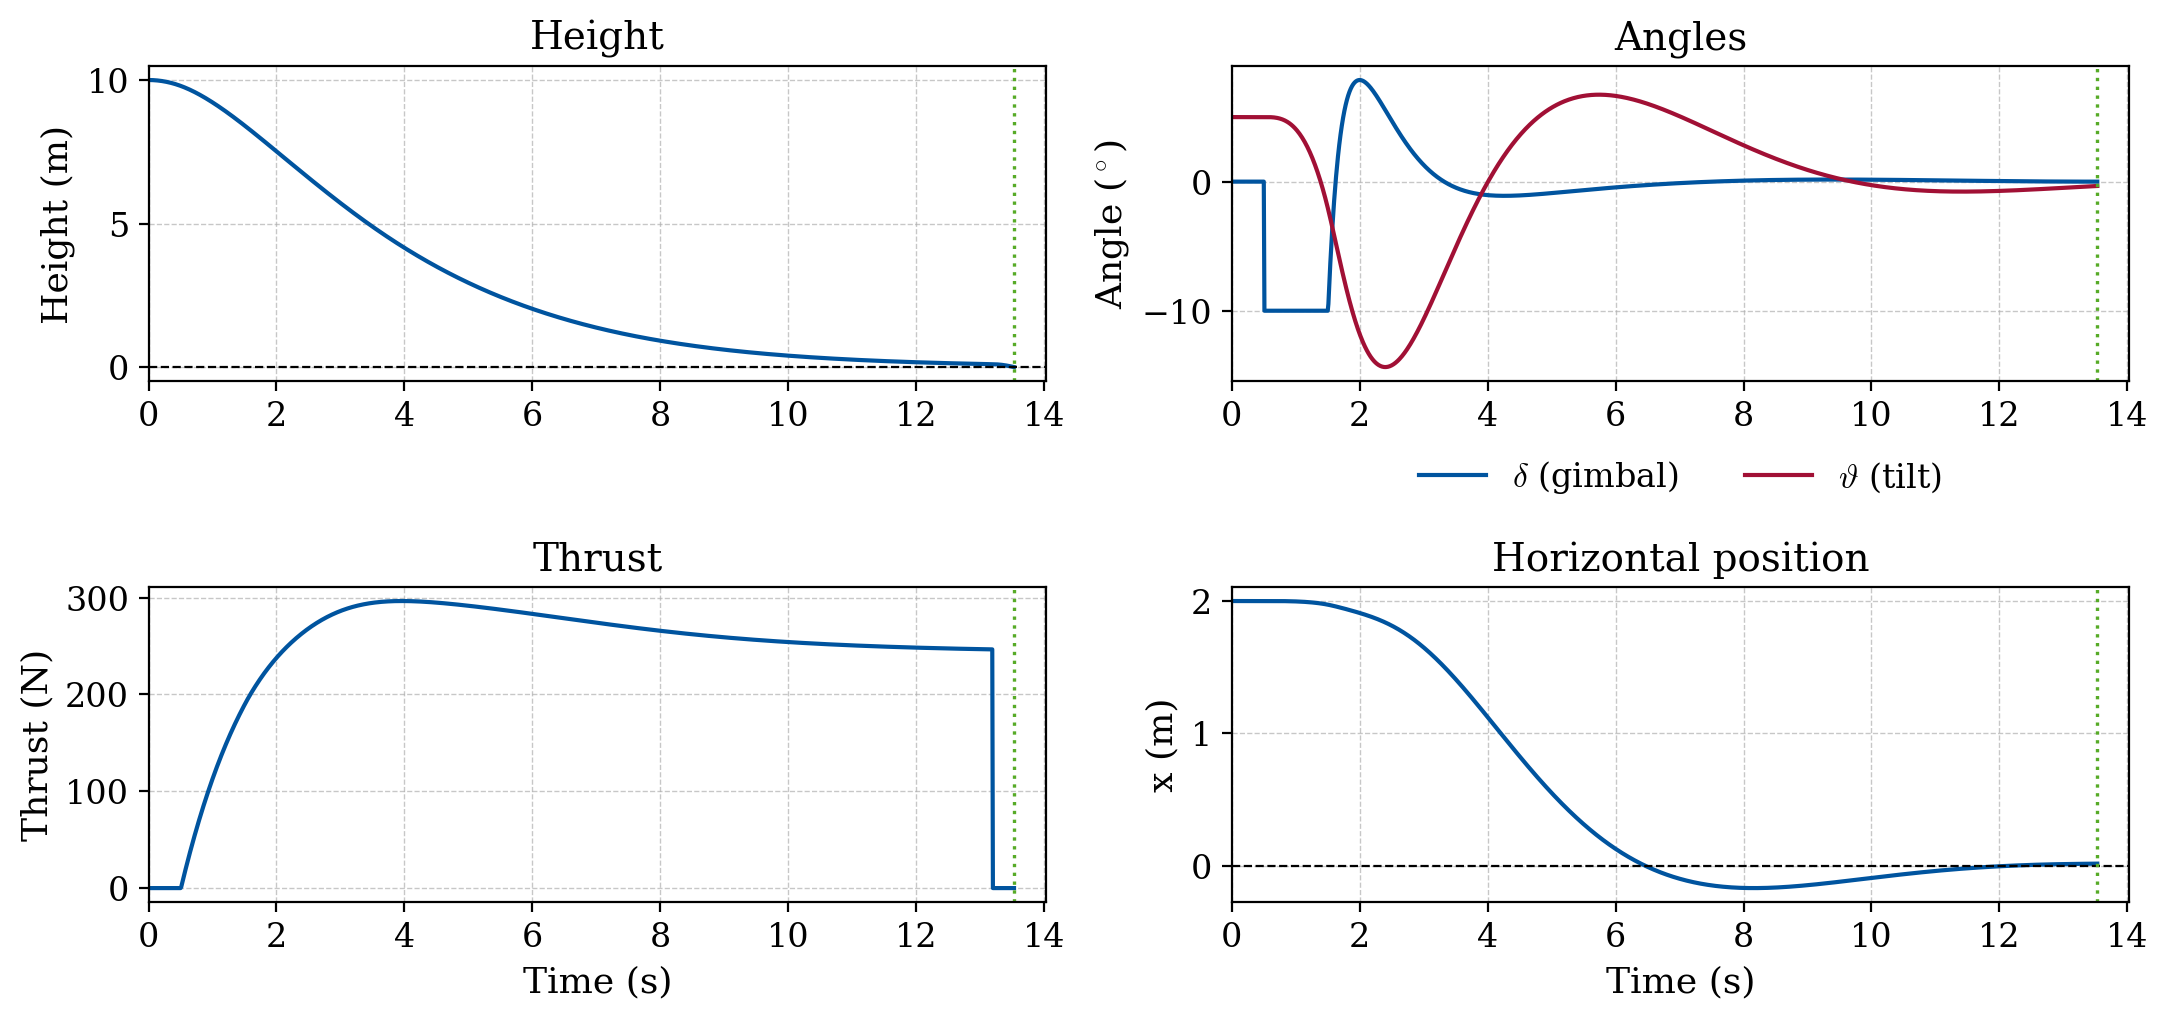
\includegraphics[width=0.96\linewidth]{figures/hopper_work.png}
\caption{\textbf{Working case} ($x_0=2~\mathrm{m}$, $\vartheta_0=5^\circ$). Touchdown at $t=13.5~\mathrm{s}$: $x=+0.02~\mathrm{m}$, $v_x=+0.01~\mathrm{m/s}$, $v_z=-0.58~\mathrm{m/s}$, $\vartheta=-0.3^\circ$ - a soft landing. Dotted green line marks touchdown; plots are truncated there.}
\label{fig:work}
\end{figure}

\begin{figure}[H]
\centering
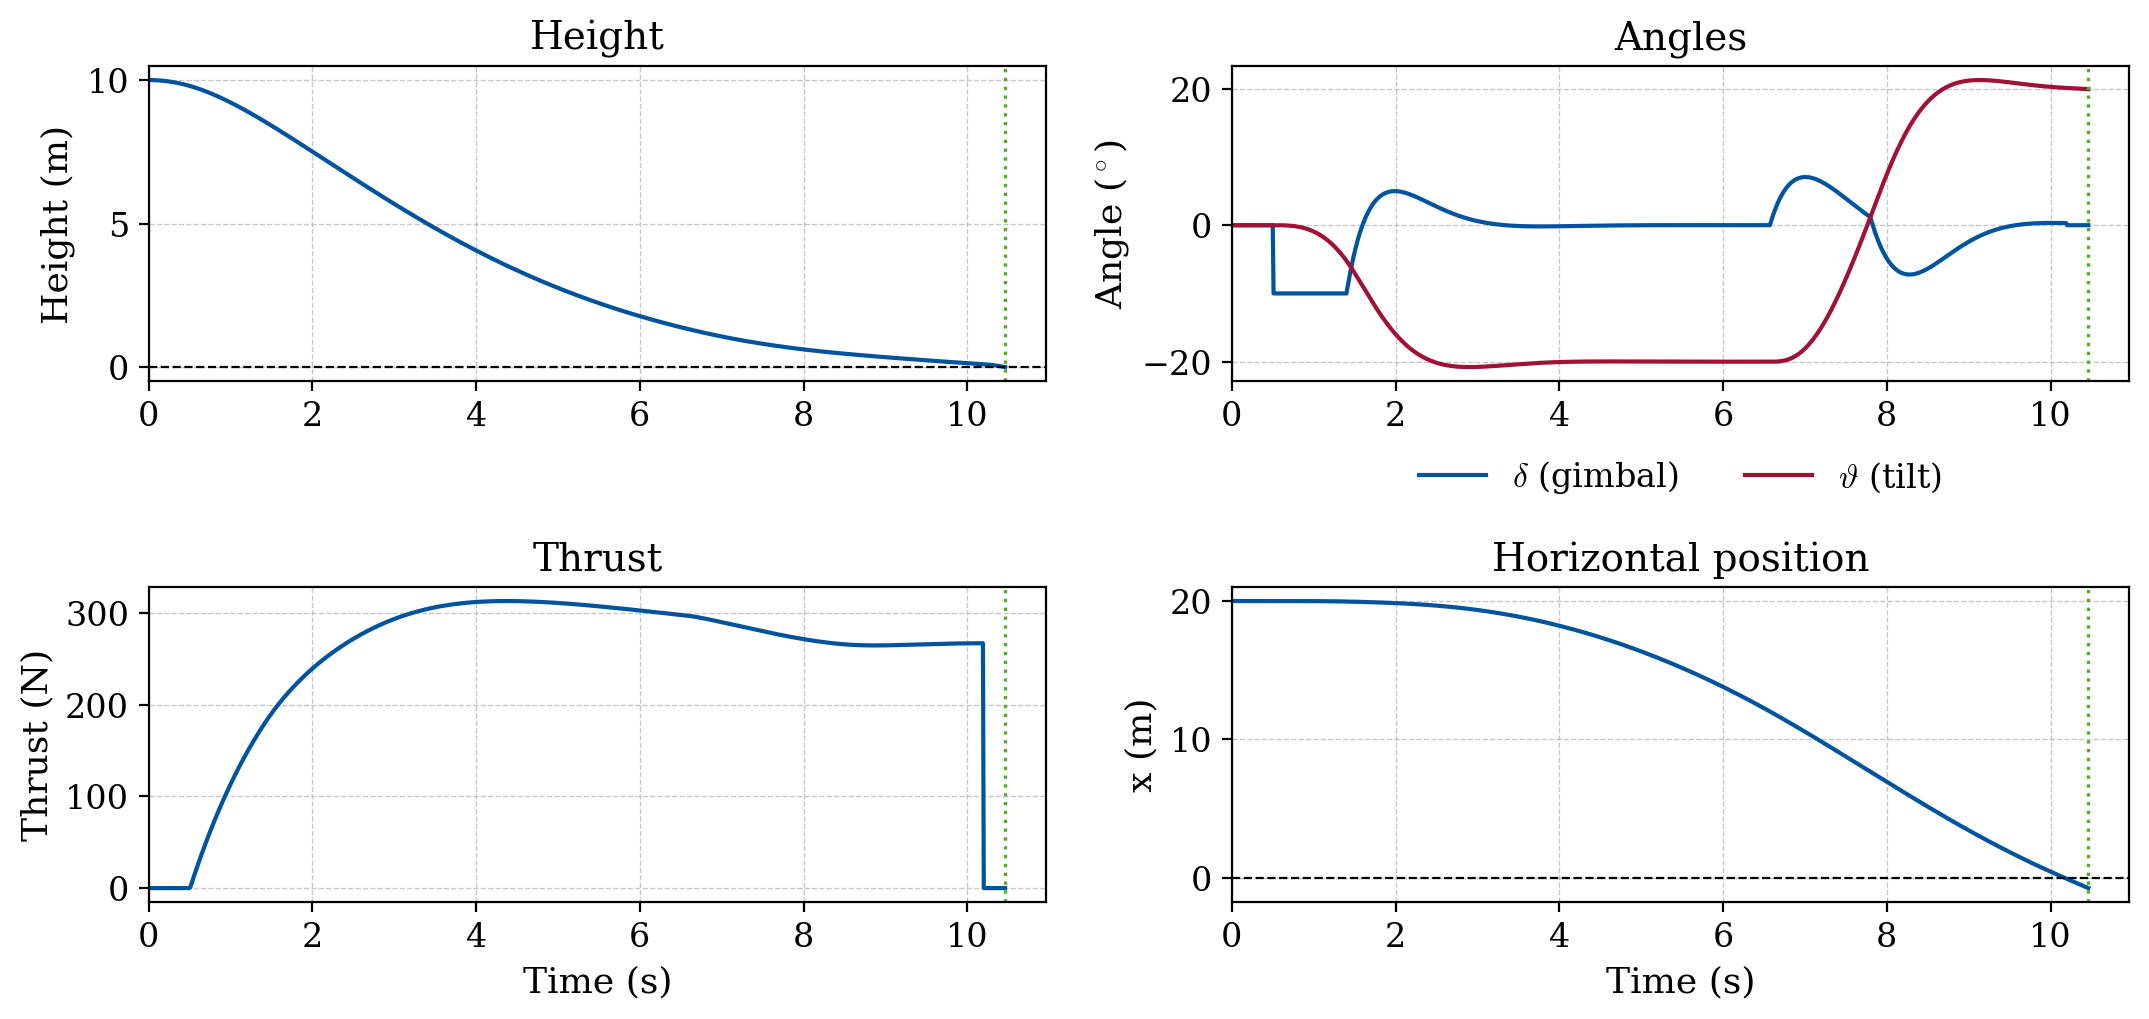
\includegraphics[width=0.96\linewidth]{figures/hopper_fail.png}
\caption{\textbf{Failing case} ($x_0=20~\mathrm{m}$). The commanded tilt saturates at $-20^\circ$ to recover the offset; touchdown at $t=10.5~\mathrm{s}$ with $v_x=-2.5~\mathrm{m/s}$ and $\vartheta=+20^\circ$ - a crash. The lateral-recovery maneuver outlasts the descent.}
\label{fig:fail}
\end{figure}

\section*{Monte Carlo dispersion analysis}

To make a claim on the quality of the controller, we look at $N=1000$ descents, where the initial conditions are chosen uniform from the following intervals: $x_0\in[-5,5]~\mathrm{m}$, $\dot x_0\in[-2,2]~\mathrm{m/s}$, $\dot z_0\in[-3,0]~\mathrm{m/s}$, $\vartheta_0\in[-10^\circ,10^\circ]$, $\omega_0\in[-3^\circ,3^\circ]/\mathrm{s}$, all from $z_0=10~\mathrm{m}$. 

We consider a landing as:
\begin{itemize}
	\item Soft: $|x|<0.5~\mathrm{m}$, $|v_x|<0.5~\mathrm{m/s}$, $|v_z|<1~\mathrm{m/s}$, $|\vartheta|<5^\circ$
	\item Acceptable: $|x|<1~\mathrm{m}$, $|v_x|<1.0~\mathrm{m/s}$, $|v_z|<2~\mathrm{m/s}$, $|\vartheta|<10^\circ$, excluding soft limits
\end{itemize} 

Of the 1000 cases, \textbf{830 (83.0\,\%) were soft} and 52 acceptable, thus \textbf{882 (88.2\,\%) within tolerance} and \textbf{118 (11.8\,\%) failures}. Failures mostly stem from large $\vartheta$ at touchdown. In Figure~\ref{fig:mc} Right, we can see that the lateral velocities at touchdown are within the $|v_x|<1$~m/s. However, the failing cases always have touchdown tilts above $|\vartheta|>10^\circ$. Contrary to the expectation, this does not stem from large initial tilts but from strong initial lateral offsets and velocities, as seen in the left figure of Figure~\ref{fig:mc}. While the initial tilts can be corrected quickly, to correct the lateral offsets, a stronger tilt needs to be set, which then is not corrected fast enough at landing.

\begin{figure}[H]
\centering
\begin{minipage}{0.49\linewidth}\centering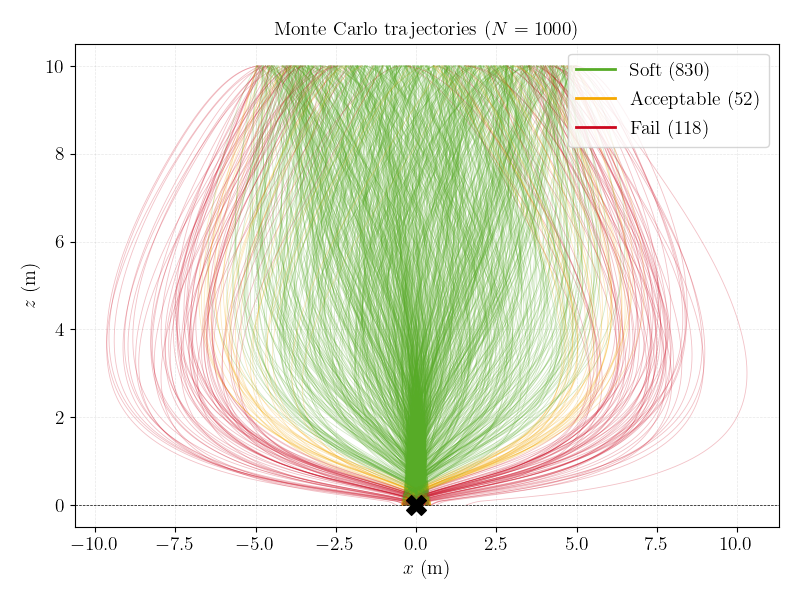
\includegraphics[width=\linewidth]{figures/Figure_1.png}\end{minipage}\hfill
\begin{minipage}{0.49\linewidth}\centering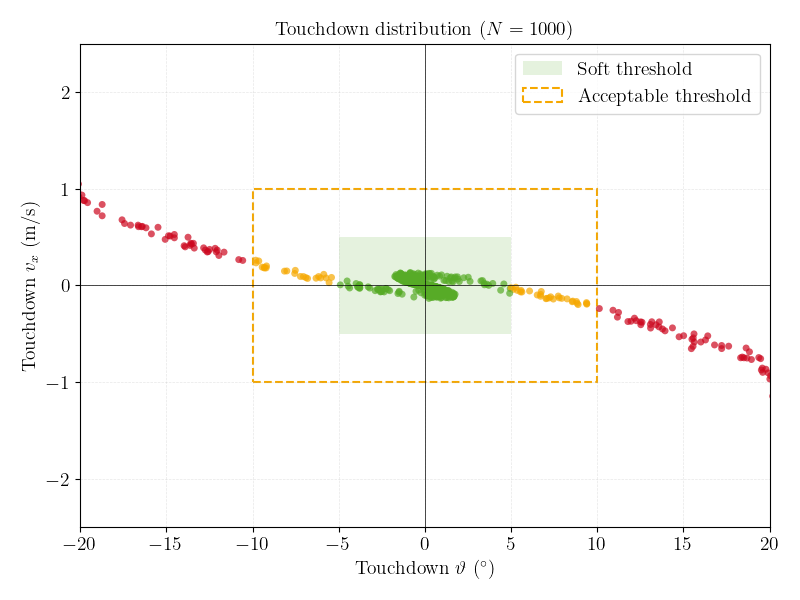
\includegraphics[width=\linewidth]{figures/Figure_2.png}\end{minipage}
\caption{Monte Carlo ($N=1000$). \textbf{Left:} trajectories, coloured by outcome. \textbf{Right:} touchdown distribution in the $\vartheta-v_x$-plane; shaded and dashed regions indicate the soft and acceptable limits, and marker colour reflects the classification. The diagonal shift stems from the tilt-lateral-velocity coupling from steering $x$ through $\vartheta$.}
\label{fig:mc}
\end{figure}

\section*{Limitations and Possible Improvements}
As a two-day study, this is meant only to build an intuition on control systems, and its limits point straight at the methods it does not use. Currently, the lander is reactive in the sense that it regulates the errors as they appear, without doing trajectory planning or fuel optimization. The system rather builds on the premise that the offsets can be corrected for before landing takes place.

The next step would be to create an optimization-based guidance system, such that fuel, actuator, and state limits enter as explicit constraints. This would allow for dealing with the large-offset regime by planning the trajectory rather than being reactive. This way, touchdown limits are met by construction and not checked afterwards. 

The step from going from a reactive robustness towards a designed-in robustness is the direction I would like to work on.



\vspace{2pt}
{\footnotesize\itshape This Project was implemented in Python (NumPy) using an RK4 propagator and a fixed random seed.}
\end{document}
